\begin{frame}\frametitle{Работа поля вдоль линии}
	За точку $A$ возьмем $(0, 1)$ за $B - (0.125, 0.5)$
	Работа поля $H$ вдоль векторной линии через это поле равна: 
	\begin{align*}
		\int\limits_{AB} \vec H \, d \vec s
		 & =
		U(B) - U(A)
		=
		(B_x + \frac{1}{B_y}) - (A_x + \frac{1}{A_y}) = \\
		 & = (0.125 + \frac{1}{0.5}) - (0 + \frac{1}{1}) = 1.125
		\label{eq:work_across_line}
	\end{align*}
	\begin{figure}
		\centering
		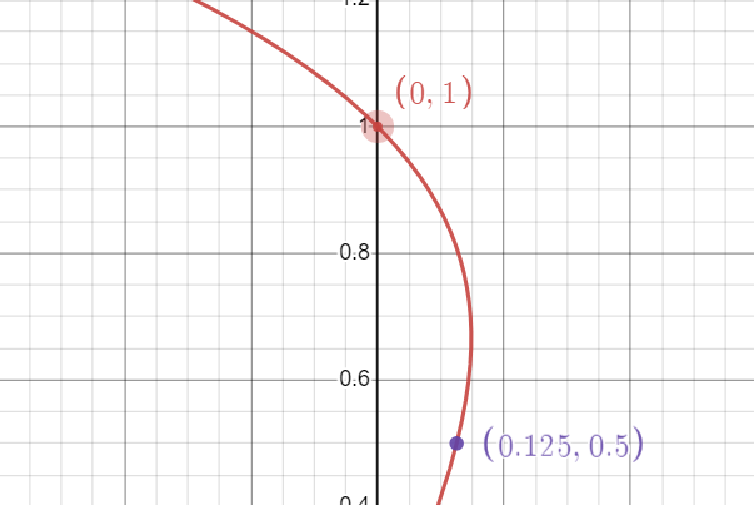
\includegraphics[width=0.5\textwidth]{figures/potential_work.pdf}
		\caption{Работа вдоль линии}\label{fig:potential_work}
	\end{figure}
\end{frame}
